\documentclass[a4paper, man, floatsintext]{apa6}
\usepackage{lmodern}
\usepackage{amssymb,amsmath}
\usepackage{ifxetex,ifluatex}
\usepackage{fixltx2e} % provides \textsubscript
\ifnum 0\ifxetex 1\fi\ifluatex 1\fi=0 % if pdftex
  \usepackage[T1]{fontenc}
  \usepackage[utf8]{inputenc}
\else % if luatex or xelatex
  \ifxetex
    \usepackage{mathspec}
  \else
    \usepackage{fontspec}
  \fi
  \defaultfontfeatures{Ligatures=TeX,Scale=MatchLowercase}
\fi
% use upquote if available, for straight quotes in verbatim environments
\IfFileExists{upquote.sty}{\usepackage{upquote}}{}
% use microtype if available
\IfFileExists{microtype.sty}{%
\usepackage{microtype}
\UseMicrotypeSet[protrusion]{basicmath} % disable protrusion for tt fonts
}{}
\usepackage{hyperref}
\hypersetup{unicode=true,
            pdfauthor={Jana B. Jarecki},
            pdfborder={0 0 0},
            breaklinks=true}
\urlstyle{same}  % don't use monospace font for urls
\usepackage{graphicx,grffile}
\makeatletter
\def\maxwidth{\ifdim\Gin@nat@width>\linewidth\linewidth\else\Gin@nat@width\fi}
\def\maxheight{\ifdim\Gin@nat@height>\textheight\textheight\else\Gin@nat@height\fi}
\makeatother
% Scale images if necessary, so that they will not overflow the page
% margins by default, and it is still possible to overwrite the defaults
% using explicit options in \includegraphics[width, height, ...]{}
\setkeys{Gin}{width=\maxwidth,height=\maxheight,keepaspectratio}
\IfFileExists{parskip.sty}{%
\usepackage{parskip}
}{% else
\setlength{\parindent}{0pt}
\setlength{\parskip}{6pt plus 2pt minus 1pt}
}
\setlength{\emergencystretch}{3em}  % prevent overfull lines
\providecommand{\tightlist}{%
  \setlength{\itemsep}{0pt}\setlength{\parskip}{0pt}}
\setcounter{secnumdepth}{0}
% Redefines (sub)paragraphs to behave more like sections
\ifx\paragraph\undefined\else
\let\oldparagraph\paragraph
\renewcommand{\paragraph}[1]{\oldparagraph{#1}\mbox{}}
\fi
\ifx\subparagraph\undefined\else
\let\oldsubparagraph\subparagraph
\renewcommand{\subparagraph}[1]{\oldsubparagraph{#1}\mbox{}}
\fi

%%% Use protect on footnotes to avoid problems with footnotes in titles
\let\rmarkdownfootnote\footnote%
\def\footnote{\protect\rmarkdownfootnote}

%%% Change title format to be more compact
\usepackage{titling}

% Create subtitle command for use in maketitle
\providecommand{\subtitle}[1]{
  \posttitle{
    \begin{center}\large#1\end{center}
    }
}

\setlength{\droptitle}{-2em}

  \title{}
    \pretitle{\vspace{\droptitle}}
  \posttitle{}
    \author{Jana B. Jarecki}
    \preauthor{\centering\large\emph}
  \postauthor{\par}
      \predate{\centering\large\emph}
  \postdate{\par}
    \date{03 Oktober, 2019}

\usepackage{natbib} \usepackage{threeparttable} \usepackage{booktabs}
\shorttitle{test} \usepackage{setspace}
\AtBeginEnvironment{tabular}{\singlespacing} \usepackage{times}
\usepackage{changes} \definechangesauthor[name={JJ}, color=orange]{jj}
\usepackage{upgreek} \AtBeginDocument{\let\maketitle\relax}

\begin{document}

\subsection{Evaluations of Gambles by Condition and Sample Size}

Table \ref{tab:means_study1} shows participants' evaluations of the
gambles in the experience and description conditions. In the experience
condition it seems that sample size has no influence on evaluations. In
the best-fitting mixed regression model \(\mathrm{M}\textsubscript{0}\)
sample size was a random effect, and gamble type---p-bet vs. \$-bet---a
fixed effect, resulting in higher evaluations of the p-bets (gamble IDs
1 to 3) compared to the \$-bets (IDs 4 to 6). This model outperformed a
model with sample size as fixed effect (\(BF\textsubscript{01} = 409\)),
and a model with a sample-size\(\times\)gamble-type interaction
(\(BF\textsubscript{01} > 1,000\)). Although this suggests that sample
size does not reliably influence the evaluations of gambles in a
decision from experience paradigm, the cognitive modeling analyses will
show a more nuanced picture.

\begin{table}[tbp]
\begin{center}
\begin{threeparttable}
\caption{\label{tab:means_study1}Valuations of Gambles in Study 1}
\begin{tabular}{lccccrr}
\toprule
Condition & Sample size category & Effective sample size & \textit{Med} & \textit{M} & D--E & D--E:$BF\textsubscript{10}$\\
\midrule
Gamble ID 1 &  &  &  &  &  & \\
\ \ \ E & xs & 5 & 5.00 & 5.16 & -0.56 & 4\\
\ \ \ E & s & 10 & 4.55 & 5.30 & -0.70 & 68\\
\ \ \ E & m & 15 & 5.00 & 5.34 & -0.74 & 24\\
\ \ \ E & l & 30 & 5.00 & 5.29 & -0.69 & 165\\
\ \ \ D & -- & -- & 4.00 & 4.60 & -- & --\\
Gamble ID 2 &  &  &  &  &  & \\
\ \ \ E & xs & 6 & 4.00 & 4.33 & -0.71 & 130\\
\ \ \ E & s & 12 & 4.00 & 4.31 & -0.69 & 609\\
\ \ \ E & m & 18 & 4.00 & 4.04 & -0.43 & 5\\
\ \ \ E & l & 36 & 4.00 & 3.99 & -0.37 & 2\\
\ \ \ D & -- & -- & 3.00 & 3.61 & -- & --\\
Gamble ID 3 &  &  &  &  &  & \\
\ \ \ E & xs & 7 & 6.00 & 7.56 & -0.99 & 4\\
\ \ \ E & s & 14 & 6.70 & 8.40 & -1.83 & 872\\
\ \ \ E & m & 21 & 6.20 & 7.92 & -1.35 & 135\\
\ \ \ E & l & 42 & 6.00 & 7.68 & -1.11 & 40\\
\ \ \ D & -- & -- & 5.00 & 6.57 & -- & --\\
Gamble ID 4 &  &  &  &  &  & \\
\ \ \ E & xs & 5 & 3.00 & 2.80 & 0.28 & >1000\\
\ \ \ E & s & 10 & 3.20 & 2.91 & 0.16 & 3\\
\ \ \ E & m & 15 & 3.00 & 2.80 & 0.28 & 55\\
\ \ \ E & l & 30 & 3.00 & 2.95 & 0.13 & 1\\
\ \ \ D & -- & -- & 3.20 & 3.08 & -- & --\\
Gamble ID 5 &  &  &  &  &  & \\
\ \ \ E & xs & 6 & 2.00 & 1.77 & 0.10 & 8\\
\ \ \ E & s & 12 & 2.00 & 1.75 & 0.12 & 14\\
\ \ \ E & m & 18 & 2.00 & 1.73 & 0.14 & 28\\
\ \ \ E & l & 36 & 2.00 & 1.81 & 0.06 & 1\\
\ \ \ D & -- & -- & 2.00 & 1.87 & -- & --\\
Gamble ID 6 &  &  &  &  &  & \\
\ \ \ E & xs & 7 & 4.00 & 3.46 & 0.18 & 3\\
\ \ \ E & s & 14 & 4.00 & 3.55 & 0.09 & 0\\
\ \ \ E & m & 21 & 4.00 & 3.58 & 0.06 & 0\\
\ \ \ E & l & 42 & 4.00 & 3.70 & -0.06 & 0\\
\ \ \ D & -- & -- & 4.00 & 3.64 & -- & --\\
\bottomrule
\addlinespace
\end{tabular}
\begin{tablenotes}[para]
\normalsize{\textit{Note.} \textit{M} = mean, \textit{Med} = median, D--E = difference between mean description-based valuations and experience-based valuations, $BF\textsubscript{10}$ = Bayes Factor quantifying the evidence for a linear model $\mathrm{M}\textsubscript{1}$ predicting that valuations differ between description and experience over a linear model $\mathrm{M}\textsubscript{0}$ predicting no such differences; both models models contain a by-participant random effect. Gambles IDs 1, 2, and 3 are \$-bets; Gamble IDs 4, 5, and 6 are p-bets.}
\end{tablenotes}
\end{threeparttable}
\end{center}
\end{table}

\subsection{Cognitive modeling of experience-based evaluations}

We used computational modeling to analyze the role of sample size in
value judgments more closely. We compared the performance of the
\added[id=jj]{relative frequency} (RF) model and the
\added[id=jj]{Bayesian value updating} (BVU) model.
\added[id=jj]{The models were compared to a baseline model, which predicts a constant evaluation equal to the mean individual evaluation. Sensible models are expected to outperform this baseline model.}

\subsubsection{Modeling Procedure} 
\added[id=jj]{The observed and predicted evaluations were normalized to a common range (range 0 - 1, by division through the gain magnitude). Maximum likelihood was used to estimate the free model parameters at the participant level, assuming observations follow a truncated normal distribution around the model predictions (truncated between 0 and 1) with a constant standard deviation ($\sigma$), that was estimated as a free parameter ($0 < \sigma \leq 1$).  Therefore, the relative frequency model had 2 free parameter, the power utility exponent $\alpha$ ($0 \leq \alpha \leq 20$) and $\sigma$. The Bayesian value updating model had 4 free parameter the gain prior $\theta_G$ ($0 \leq \theta_G \leq 1$), the learning rate $\delta$ ($0 \leq \delta \leq 10$), $\alpha$ and $\sigma$; the loss prior was constrained $\theta_0=2-\theta_G$. The baseline model had 2 free parameter, the mean evaluation $\mu$ and $\sigma$. We estimated the parameters using an augmented Lagrange multiplier method \citep[Rsolnp package, version 1.16]{Ghalanos2015}. We compared the models by their evidence strength and BIC weights on the Bayesian information criterion (BIC) \cite[evidence in favor of a model compared to the individually best-fitting model][]{Kass1995, Lewandowsky2011}. Higher weights indicate stronger evidence for a model.}

\subsubsection{Modeling Results}
\added[id=jj]{We will first outline the quantitative model fit, followed by the qualitative model fit, and lastly analyze the effects of sample size given the cognitive strategies.}

\textit{Quantitative Model Fit.} The Bayesian value updating model
described the majority of the participants best (30 of 40; 75\%). The
relative frequency model described 9 participants best (22\%); the
baseline model described only 1 participants best. Figure
\ref{fig:study1_model_weights} shows the evidence strength for the
models by participant. The models' mean Bayesian information criterion
across all participants equaled BIC\textsubscript{BVU}\(= -124\),
BIC\textsubscript{RF}\(= -110\), and BIC\textsubscript{BASE}\(= -17\)
(lower values indicate better fit).

\begin{figure}[htb]

{\centering 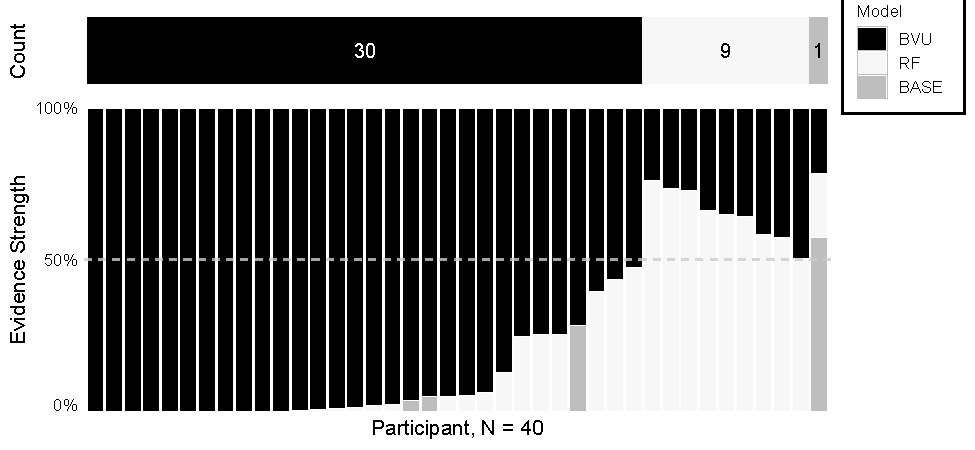
\includegraphics{../figures/study1_model_weights-1} 

}

\caption{Evidence for the models for individual participants. \textit{RF}$=$ relative frequency model, \textit{BVU}$=$ Bayesian value updating model, \textit{BASE}$=$ Baseline model.}\label{fig:study1_model_weights}
\end{figure}

\added[id=jj]{
The estimated parameter of the winning models, which Table \ref{tab:study1_parameter} summarizes, reveal that the power utility exponent ($\alpha$) is almost identical for the participants using a Bayesian value updating strategy ($M_{\alpha}= 1.43$) and those using a relative frequency strategy ($M_{\alpha}=1.60$), $M = -0.13$ 95\% HDI $[-0.71$, $0.38]$, $\mathrm{BF}_{\textrm{01}} = 3.26$. Participants using the Bayesian strategy had, on average, a prior belief that gains occur with 46\% (gain prior $\theta_G = 0.92$; zero-outcome prior $\theta_0 = 1.08$). Also, their estimated learning rate $\delta$ was anti-conservative ($M_{\delta}=1.36$; values $>$ 1 are liberal, 1 is optimal Bayesian, $<$ 1 is conservative learning); this contradicts previous results that found conservative learners \citep{Edwards1967,Tauber2017}, but the liberal learning in our task can be explained because participants repeatedly sampled from the same set of gambles.
}

\begin{table}[tbp]
\begin{center}
\begin{threeparttable}
\caption{\label{tab:study1_parameter}Parameter Estimates of Winning Models, \textit{M (SD)}}
\begin{tabular}{lccccc}
\toprule
Winning Model & $\alpha$ & $\delta$ & $\theta_G$ & $\mu$ & $\sigma$\\
\midrule
BVU (\textit{n}$=$30) & 1.49 (1.47) & 1.36 (2.12) & 0.92 (0.66) & -- & 0.13 (0.07)\\
RF (\textit{n}$=$9) & 1.61 (0.58) & -- & -- & -- & 0.12 (0.02)\\
BASE (\textit{n}$=$1) & -- & -- & -- & 0.47 (NA) & 0.30 (NA)\\
\bottomrule
\addlinespace
\end{tabular}
\begin{tablenotes}[para]
\normalsize{\textit{Note.} \textit{BVU}$=$ Bayesian value updating model, \textit{RF}$=$ relative frequency model, \textit{BASE}$=$baseline model. Parameters denote: $\alpha=$ power utility exponent, $\theta_G$ gain prior, $\mu=$ mean evaluation, $\sigma$ standard deviation.}
\end{tablenotes}
\end{threeparttable}
\end{center}
\end{table}

\textit{Qualitative Model Fit.}
\added[id=jj]{The qualitative fit between the models and the data is shown in Figure \ref{fig:ind_fits1}, which plots the predictions of the best-fitting models against the observed evaluations. It shows that the models generally describe the data well (mean $r\textsubscript{pred,obs} = 0.71$), except in four cases, where even the winning model fails to resemble the data qualitatively (participants number 05, 19, 24, 38, with $r\textsubscript{pred,obs} < 0.40$). For these cases, for whom the winning model is the Bayesian updating model, the model must be rejected because of qualitative mis-fit.}

\begin{figure}[htb]

{\centering 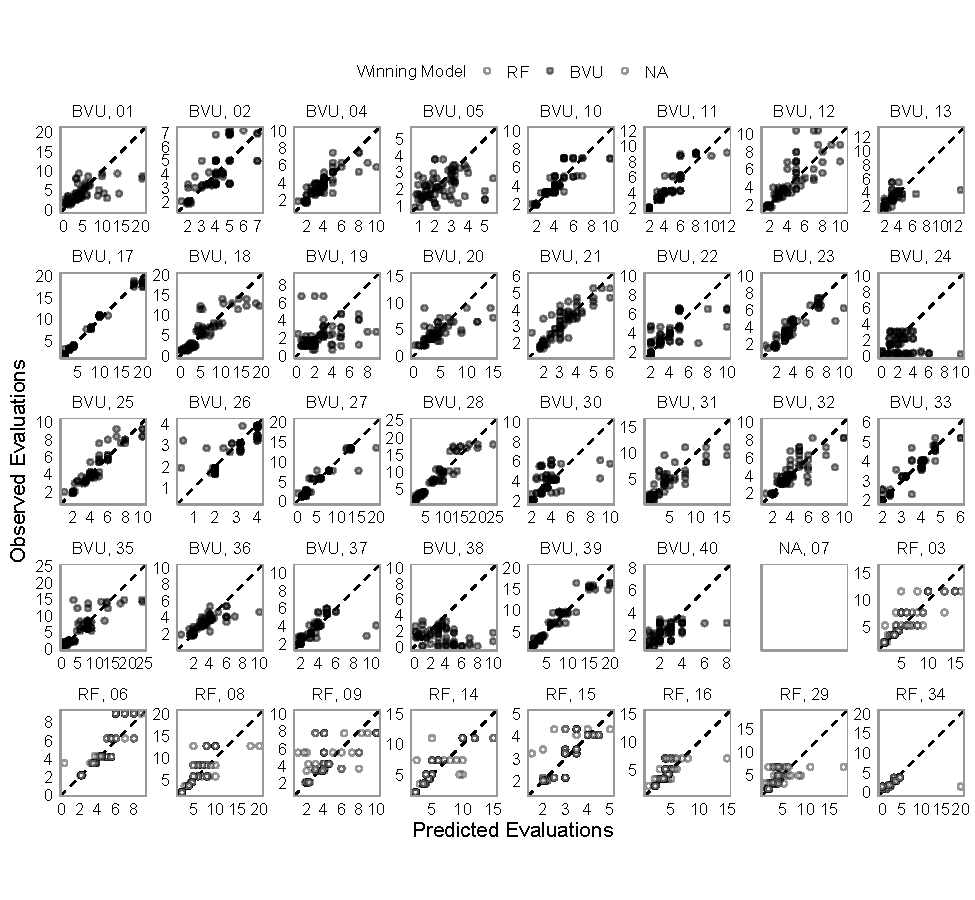
\includegraphics{../figures/ind_fits1-1} 

}

\caption{Predicted evaluations from the best-fitting models plotted against the observed evaluations (by participant). \textit{BVU}$=$ Bayesian value updating model, \textit{RF}$=$ relative frequency model, \textit{BASE}$=$baseline model.}\label{fig:ind_fits1}
\end{figure}

\added[id=jj]{The cognitive modeling results thus show that most participants used a Bayesian strategy, and some used a relative-frequency strategy. This strategy heterogeneity helps understanding the behavioral null finding---that sample size seemed to have no effect on valuations---that were observed at the aggregate level (Table \ref{tab:means_study1}). The aggregate analysis fails to take the individual differences in learning strategies into account, while participants are best described by a mixture of strategies. Moreover, the aggregate analysis also fails to account for differences in the prior beliefs about gain probabilities. Depending on the prior belief, the Bayesian value updating (BVU) model predicts either a decrease or an increase in valuations with increasing sample size. The next analysis will focus on these differences.}

\emph{The effect of sample size given cognitive strategies.} Next, we
qualitatively analyzed if sample size differentially affects the
relative-frequency-type and Bayesian-type learners. We expected that
sample size leads to changes in the evaluations of the Bayesian learners
depending on their priors, and that sample size does not affect the
evaluations of the relative-frequency learners. \added[id=jj]{
The Bayesian model predicts that sample size changes the evaluations differently as a function of prior beliefs. Participants with a gain prior---initially believing that gains are more likely than zero-outcomes---should decrease the evaluations of \$-bets as sample sizes increase, because participants overwrite their priors through sampling and learn that gains of \$-bets are less likely than zero-outcomes. By contrast, participants with a zero-outcome prior---initially believing that zero-outcomes are more likely than gains---should increase their evaluations of p-bets as sample size increases, because they learn that gains of p-bets are more likely than zero-outcomes (see the probabilities in Table~\ref{table:Lotteries}).
}

\textbackslash{}added{[}id=jj{]}\{ Based on the cognitive modeling
results, participants were classified into three learner types,
relative-frequency learners, Bayesian learners with gain priors (prior
\(\theta_G > 1\)), and Bayesian learners with loss priors (prior
\(\theta_G \leq 1\)). Figure \ref{fig:qual1} shows how the learner
types' evaluations of p-bets and \$-bets change with increasing sample
size. The relative-frequency learner types evaluated both p-bets and
\$-bets quite unaffected by sample sizes, whereas the Bayesian learner
types changed their evaluations slightly with sample size in the
predicted directions. Statistical analyses by means of a Bayesian
generalized linear
model\footnote{regressing the (normalized) evaluations on the predictors sample size, gamble type (p-bet, \$-bet), and type (BVU-gain-prior, BVU-loss-prior, RF) with a by-participant random intercept; categorical predictors were effects-coded to facilitate interpretation of interactions \citep[for details, see][]{SingmannForthcoming}), however, showed no substantial support that including the learner type as predictor improves goodness of fit, $BF\textsubscript{01}=0.393419762088619FALSE$, where 0 $=$ the model including learning type and 1 $=$ the model excluding learning type.
}

\begin{figure}[htb]

{\centering 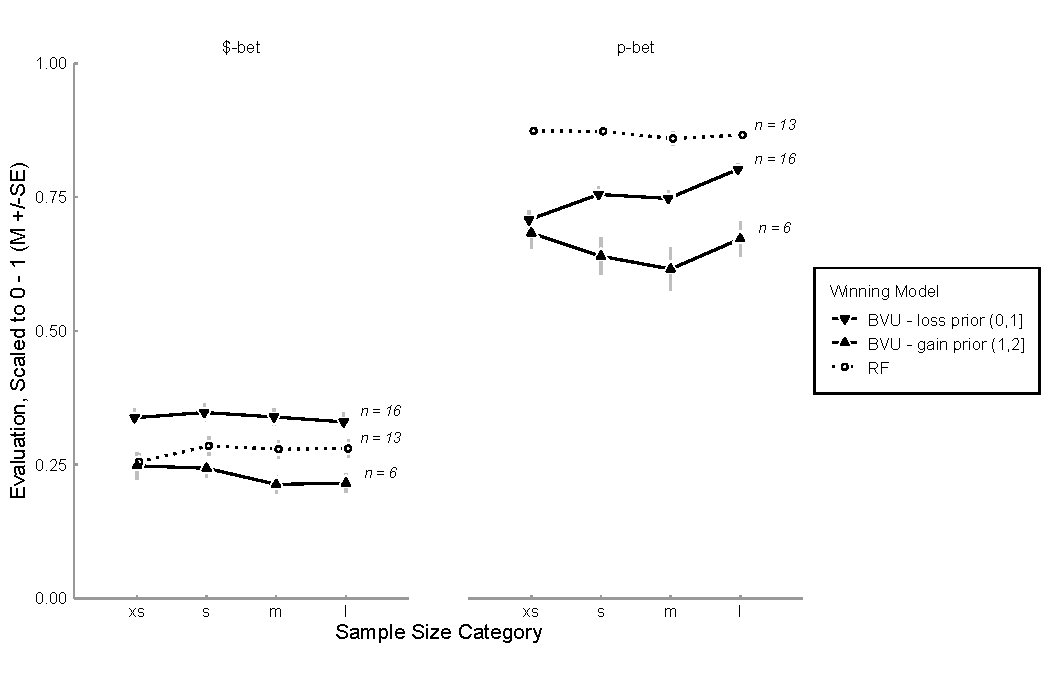
\includegraphics{../figures/qual1-1} 

}

\caption{Mean evaluation (standardized to 0 - 1) by winning model and prior beliefs of the BVU model. \textit{BVU}$=$Bayesian value updating model, \textit{RF}$=$ Relative frequency model. Error bars indicate standard errors. \textit{\$-bet}: low-probability high-outcome gambles, \textit{p-bet}: high-probability low-outcome gambles. Sample sizes (xs, x, m, l), see Table \ref{tab:Lotteries}. \textit{n=16, 13, 6} denotes the number of participants best-described by the respective models.}\label{fig:qual1}
\end{figure}

\subsubsection{Effect of gamble type and sampling order}

The mean and median evaluations of \$-bets were higher than for p-bets
(Gamble IDs 1--3 versus 4--6, Table \ref{tab:means_study1}), despite the
gambles having the same expected value. This finding is supported by
comparing a linear Bayesian regression model of gamble evaluations
\(\mathrm{M}\textsubscript{0}\)
\added[id=jj]{that includes the expected value as random effect} with a
model \(\mathrm{M}\textsubscript{1}\)
\added[id=jj]{that includes p-bets and \$-bets as fixed effects}
(\(BF\textsubscript{10} > 1,000\)).

To test for recency or primacy effects, we compared how well the first
half and the second half of the sample sequence in each trial predicts
valuations. A linear model \(\mathrm{M}\textsubscript{0}\) that predicts
valuations as a function of the random factor gamble ID outperforms a
model \(\mathrm{M}\textsubscript{1}\), which also includes the mean of
the first half of the observed samples as a fixed factor
(\(BF\textsubscript{01} = 16.6\)) and model
\(\mathrm{M}\textsubscript{2}\), which includes the mean of the second
half of observed samples (\(BF\textsubscript{02} = 6.7\)). In summary,
our analysis did not provide evidence for recency or primacy effects.

\subsubsection{Confidence ratings}

Participants' aggregated mean confidence ratings of their valuations
from experience in the extra small, small, medium, and large sample-size
categories were \(4.11\) (\(SD = 1.10\)), \(4.15\) (\(SD = 1.04\)),
\(4.14\) (\(SD = 1.03\)), and \(4.16\) (\(SD = 1.06\)) for xs, s, m, and
l (respectively). Sample size did not influence participants' confidence
systematically: \(\mathrm{M}\textsubscript{0}\), which predicts
confidence rating as a function of a random participant effect, was
strongly preferred over \(\mathrm{M}\textsubscript{1}\), which in
addition includes the sample-size category as a predictor
(\(BF\textsubscript{01} = 737\)).

\added[id=jj]{According to Bayesian value updating higher sample sizes should increase confidence. The relative frequency model predicts no influence of sample size on confidence. We analyzed the confidence ratings by best-fitting model (Bayesian-type learners and relative-frequency-type learners). The confidence of Bayesian learners did not change remarkably across sample sizes ($M=4.17, 4.09, 4.18, 4.17$ for sample sizes s, xs, l, m, respectively; $SD$s$=$ 0.99, 1.09, 1.02, 1.02, respectively). A linear model\footnote{with by-participant random intercept and the predictors effect-coded.} of the confidence ratings, which excluded sample size as predictor, was preferred over a model including sample size ($BF\textsubscript{excl,incl} = 3.01$).
  Similarly, the confidence of relative-frequency-type learners did not show an effect of sample size on confidence ratings ($M = 4.07, 4.14, 4.10, 4.10$ for sample sizes mxssl, respectively; \textit{SD}s$=$ 1.08, 1.17, 1.15, 1.20, respectively; BF\textsubscript{excl,incl}$= 0.00348182551069965FALSE$)}.

\subsubsection{Description versus experience}

The above Table \ref{tab:means_study1} shows the mean and median
valuations from description and the difference between the mean
valuations in the experience and description conditions. Further, it
provides the Bayes factors, quantifying the evidence in favor of a
difference between valuations from experience and those from
description.

Valuations made from description and experience differed for most of the
gambles and sample sizes (see Table \ref{table:meansStudy2}, rightmost
column). In particular, participants attached a higher value to
experienced than to described \$-bets (Gambles 1--3) but attached a
higher value to described than to experienced p-bets (Gambles 4--6).
Thus, we found a D--E gap that is the opposite of the classic D--E gap
observed in choice paradigms. In our study, participants valued gambles
as if they overweighted rare events from description \textit{and}
experience. This effect was even stronger when people made valuations
from experience.

We also compared participants' confidence ratings of valuations from
experience in each sample-size category to those from description
(\(M = 4.04\), \(SD = 1.08\)). Separately for each sample-size category,
we compared \(\mathrm{M}\textsubscript{0}\), which predicts confidence
as a function of random participant effects, with
\(\mathrm{M}\textsubscript{1}\), which takes condition as an additional
fixed factor into account. The analyses suggest that participants were
slightly more confident about their ratings from experience than from
description for small (\(BF\textsubscript{10} = 2.5\)), medium
(\(BF\textsubscript{10} = 1.3\)), and large
(\(BF\textsubscript{10} = 4.8\)) sample sizes. For the extra small
sample sizes (\(BF\textsubscript{10} = 0.3\)), confidence judgments did
not differ.


\end{document}
